\documentclass[aspectratio=169]{beamer}

\usepackage[utf8]{inputenc}
\usepackage[T1]{fontenc}
\usepackage[ngerman, provide=*]{babel}
\usepackage{helvet}
\renewcommand{\familydefault}{\sfdefault}
\usepackage{graphicx}
\usepackage{tikz}
\usetikzlibrary{positioning, arrows.meta, calc, decorations.pathmorphing}

% ------------------------- Farbpalette -------------------------------
\definecolor{deepsea}{HTML}{0B1F33}   % dunkler Hintergrund
\definecolor{ocean}{HTML}{0E7C86}
\definecolor{teal}{HTML}{2EC4B6}      % Akzent
\definecolor{foam}{HTML}{E8F1F2}      % Text
\definecolor{coral}{HTML}{FF6B6B}     % Warnung / "naiv"
\definecolor{amber}{HTML}{F4A259}

% ------------------------- Look & Feel -------------------------------
\setbeamertemplate{navigation symbols}{}
\setbeamercolor{background canvas}{bg=deepsea}
\setbeamercolor{normal text}{fg=foam}
\setbeamercolor{frametitle}{fg=foam}
\setbeamercolor{structure}{fg=teal}
\setbeamercolor{itemize item}{fg=teal}

\setbeamerfont{frametitle}{size=\Large, series=\bfseries}

% Frametitel mit Akzentbalken
\setbeamertemplate{frametitle}{%
  \vspace*{0.55cm}%
  \hspace*{0.7cm}{\color{teal}\rule[-0.15ex]{3.5pt}{1.05em}}\hspace{0.45em}%
  \insertframetitle\par
}

% schlanke Fusszeile mit Seitenzahl
\setbeamertemplate{footline}{%
  \hfill{\color{teal}\scriptsize \insertframenumber\,/\,\inserttotalframenumber}%
  \hspace{0.7cm}\vspace{0.35cm}%
}

% ------------------------- Metadaten ---------------------------------
\title{Echtzeit-Tsunamis}
\subtitle{Interaktive Visualisierung mit OpenGL}
\author{Mika Brückner, Yannik Köllmann, Jan Vogt}
\date{18.06.2026}

% =====================================================================
\begin{document}

% ---------- Titelframe -----------------------------------------------
\begin{frame}[plain]
  \centering
  \vspace{1.4cm}
  {\color{teal}\rule{2.2cm}{2.5pt}}\\[0.7cm]
  {\Huge\bfseries Echtzeit-Tsunamis}\\[0.45cm]
  {\large\color{foam!85} Interaktive Visualisierung mit OpenGL}\\[1.4cm]
  {\color{foam!75}\small \insertauthor}\\[0.35cm]
  {\color{foam!55}\footnotesize Tsunami Lab \quad\textbullet\quad \insertdate}
\end{frame}

% ---------- 1 | Bisher: langsam & statisch ---------------------------
\begin{frame}{Wie es bisher lief}
  \vspace{0.7cm}
  \centering
  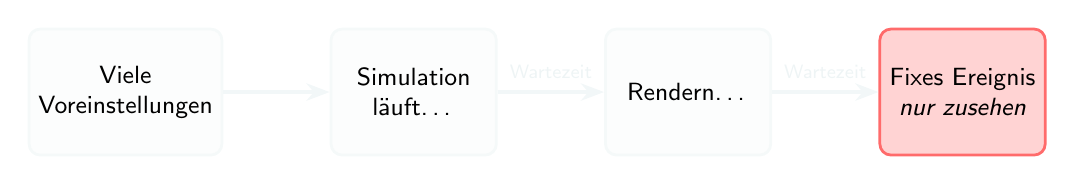
\begin{tikzpicture}[
      alt/.style={draw=foam!45, line width=1pt, rounded corners,
        fill=foam!12, text=black, align=center, font=\small,
        minimum width=2.1cm, minimum height=1.6cm},
      stop/.style={draw=coral, line width=1pt, rounded corners,
        fill=coral!30, text=black, align=center, font=\small,
        minimum width=2.1cm, minimum height=1.6cm},
      pfeil/.style={-{Stealth}, foam!55, line width=1.2pt}]
    \node[alt] (a) {Viele\\Voreinstellungen};
    \node[alt, right=1.35cm of a] (b) {Simulation\\läuft\dots};
    \node[alt, right=1.35cm of b] (c) {Rendern\dots};
    \node[stop, right=1.35cm of c] (d) {Fixes Ereignis\\\textit{nur zusehen}};
    \draw[pfeil] (a) -- (b);
    \draw[pfeil] (b) -- node[midway, above=1pt, foam!75, font=\scriptsize]{Wartezeit} (c);
    \draw[pfeil] (c) -- node[midway, above=1pt, foam!75, font=\scriptsize]{Wartezeit} (d);
  \end{tikzpicture}
  \\[1.0cm]
  {\large Viel Vorkonfiguration, spürbare \textcolor{coral}{Wartezeit}.\\[0.15cm]
   Am Ende ein \textcolor{coral}{fixes Ereignis ohne Interaktion}.}
  \note{~30s. Status quo: umstaendlich, langsam, statisch. Motiviert Echtzeit + Interaktion.}
\end{frame}

% ---------- 2 | Die Idee + Render ------------------------------------
\begin{frame}{Die Idee}
  \centering
  \vspace{0.2cm}
  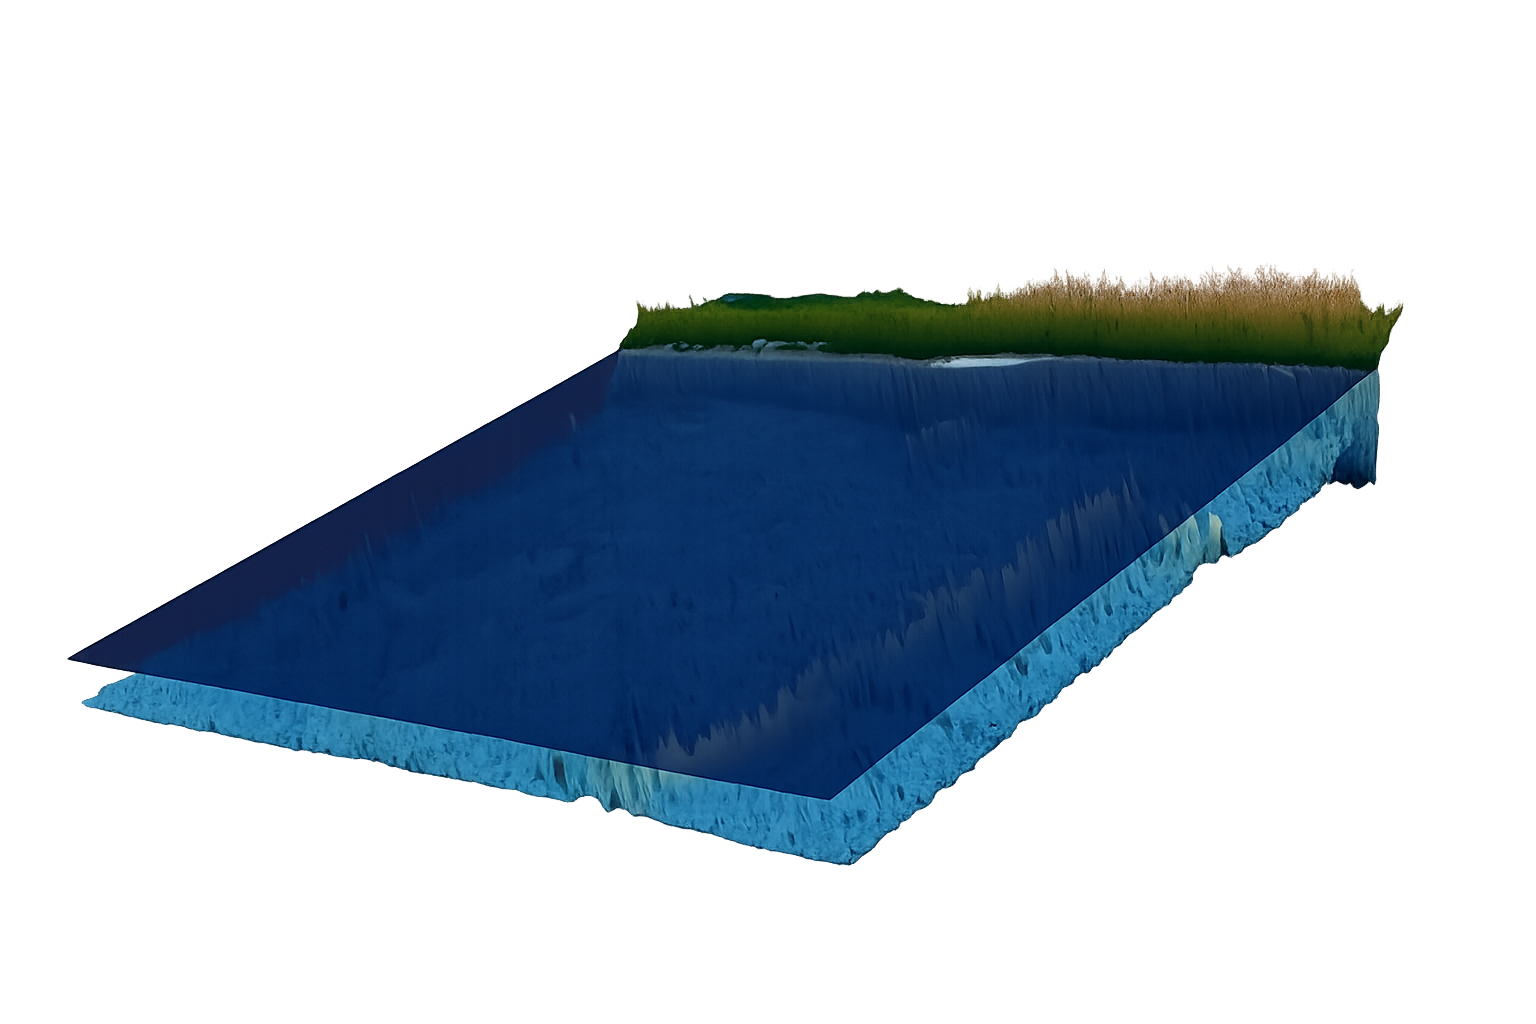
\includegraphics[width=0.5\linewidth]{render.png} \\
  {\large Diesen Solver haben wir \textcolor{teal}{bereits}.\\[0.15cm]
  Unser Projekt würde ihn in \textcolor{teal}{Echtzeit steuerbar} machen.}
  \note{~45s. Hier den vorhandenen Render zeigen. Botschaft: existiert schon, geringes Risiko.}
\end{frame}

% ---------- 3 | Die Luecke (naiv vs. Okada) --------------------------
\begin{frame}{Das Problem mit dem simplen Klick}
  \centering
  \vspace{0.2cm}
  \begin{columns}[T]
    % ---- links: naiv ----
    \begin{column}{0.48\textwidth}
      \centering
      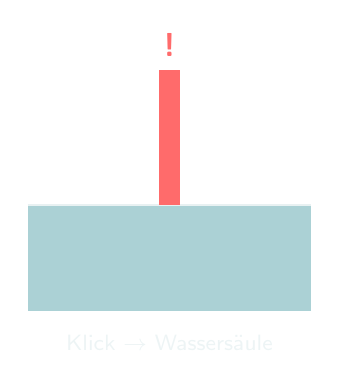
\begin{tikzpicture}[scale=0.9]
        \useasboundingbox (0,-0.75) rectangle (4,4.0);
        \fill[ocean!35] (0,0) rectangle (4,1.5);
        \draw[foam, thick] (0,1.5) -- (4,1.5);
        \fill[coral] (1.85,1.5) rectangle (2.15,3.4);
        \node[coral, font=\large\bfseries] at (2,3.75) {!};
        \node[foam!80, font=\footnotesize] at (2,-0.45) {Klick $\rightarrow$ Wassersäule};
      \end{tikzpicture}\\[0.7cm]
      {\color{coral}\bfseries Naiv}\\[0.15cm]
      {\small\color{foam!80} Unrealistisch, beliebige Stelle}
    \end{column}
    % ---- rechts: Okada ----
    \begin{column}{0.48\textwidth}
      \centering
      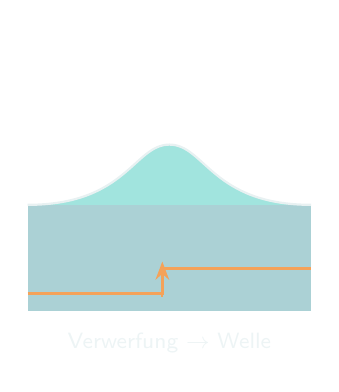
\begin{tikzpicture}[scale=0.9]
        \useasboundingbox (0,-0.75) rectangle (4,4.0);
        \fill[ocean!35] (0,0) rectangle (4,1.5);
        \draw[foam, thick, fill=teal!45]
        (0,1.5) .. controls (1.4,1.5) and (1.5,2.35) ..
        (2,2.35) .. controls (2.5,2.35) and (2.6,1.5) .. (4,1.5);
        \draw[amber, very thick] (0,0.25) -- (1.9,0.25) -- (1.9,0.6) -- (4,0.6);
        \draw[-{Stealth}, amber, thick] (1.9,0.2) -- (1.9,0.7);
        \node[foam!80, font=\footnotesize] at (2,-0.45) {Verwerfung $\rightarrow$ Welle};
      \end{tikzpicture}\\[0.7cm]
      {\color{teal}\bfseries Unser Weg (Okada-Modell)}\\[0.15cm]
      {\small\color{foam!80} Der Boden verschiebt sich, das Wasser reagiert physikalisch}
    \end{column}
  \end{columns}
  \note{~45s. Der Kontrast ist euer staerkstes Argument. Bild reden lassen.}
\end{frame}

% ---------- 4 | Die Reise (Ablauf) -----------------------------------
\begin{frame}{So fühlt sich das an}
  \vspace{0.6cm}
  \centering
  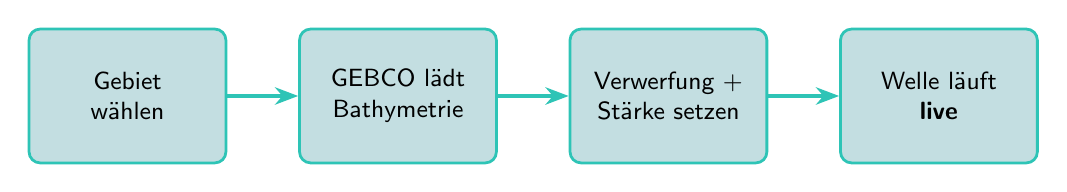
\begin{tikzpicture}[
      schritt/.style={draw=teal, line width=1pt, rounded corners,
        fill=ocean!25, text=black, align=center, font=\small,
        minimum width=2.5cm, minimum height=1.7cm},
      pfeil/.style={-{Stealth}, teal, line width=1.2pt}]
    \node[schritt] (a) {Gebiet\\wählen};
    \node[schritt, right=0.9cm of a] (b) {GEBCO lädt\\Bathymetrie};
    \node[schritt, right=0.9cm of b] (c) {Verwerfung +\\Stärke setzen};
    \node[schritt, right=0.9cm of c] (d) {Welle läuft\\\textbf{live}};
    \draw[pfeil] (a) -- (b);
    \draw[pfeil] (b) -- (c);
    \draw[pfeil] (c) -- (d);
  \end{tikzpicture}
  \\[1.0cm]
  {\large Keine Konfigurationsdatei. Der \textcolor{teal}{Ozean reagiert auf einen Klick}.}
  \note{~50s. Den Ablauf nicht vorlesen, sondern entlanggehen. Interaktivitaet betonen.}
\end{frame}

% ---------- 5 | Presets ----------------------------------------------
\begin{frame}{Verankert in der Realität}
  \centering
  \vspace{0.2cm}
  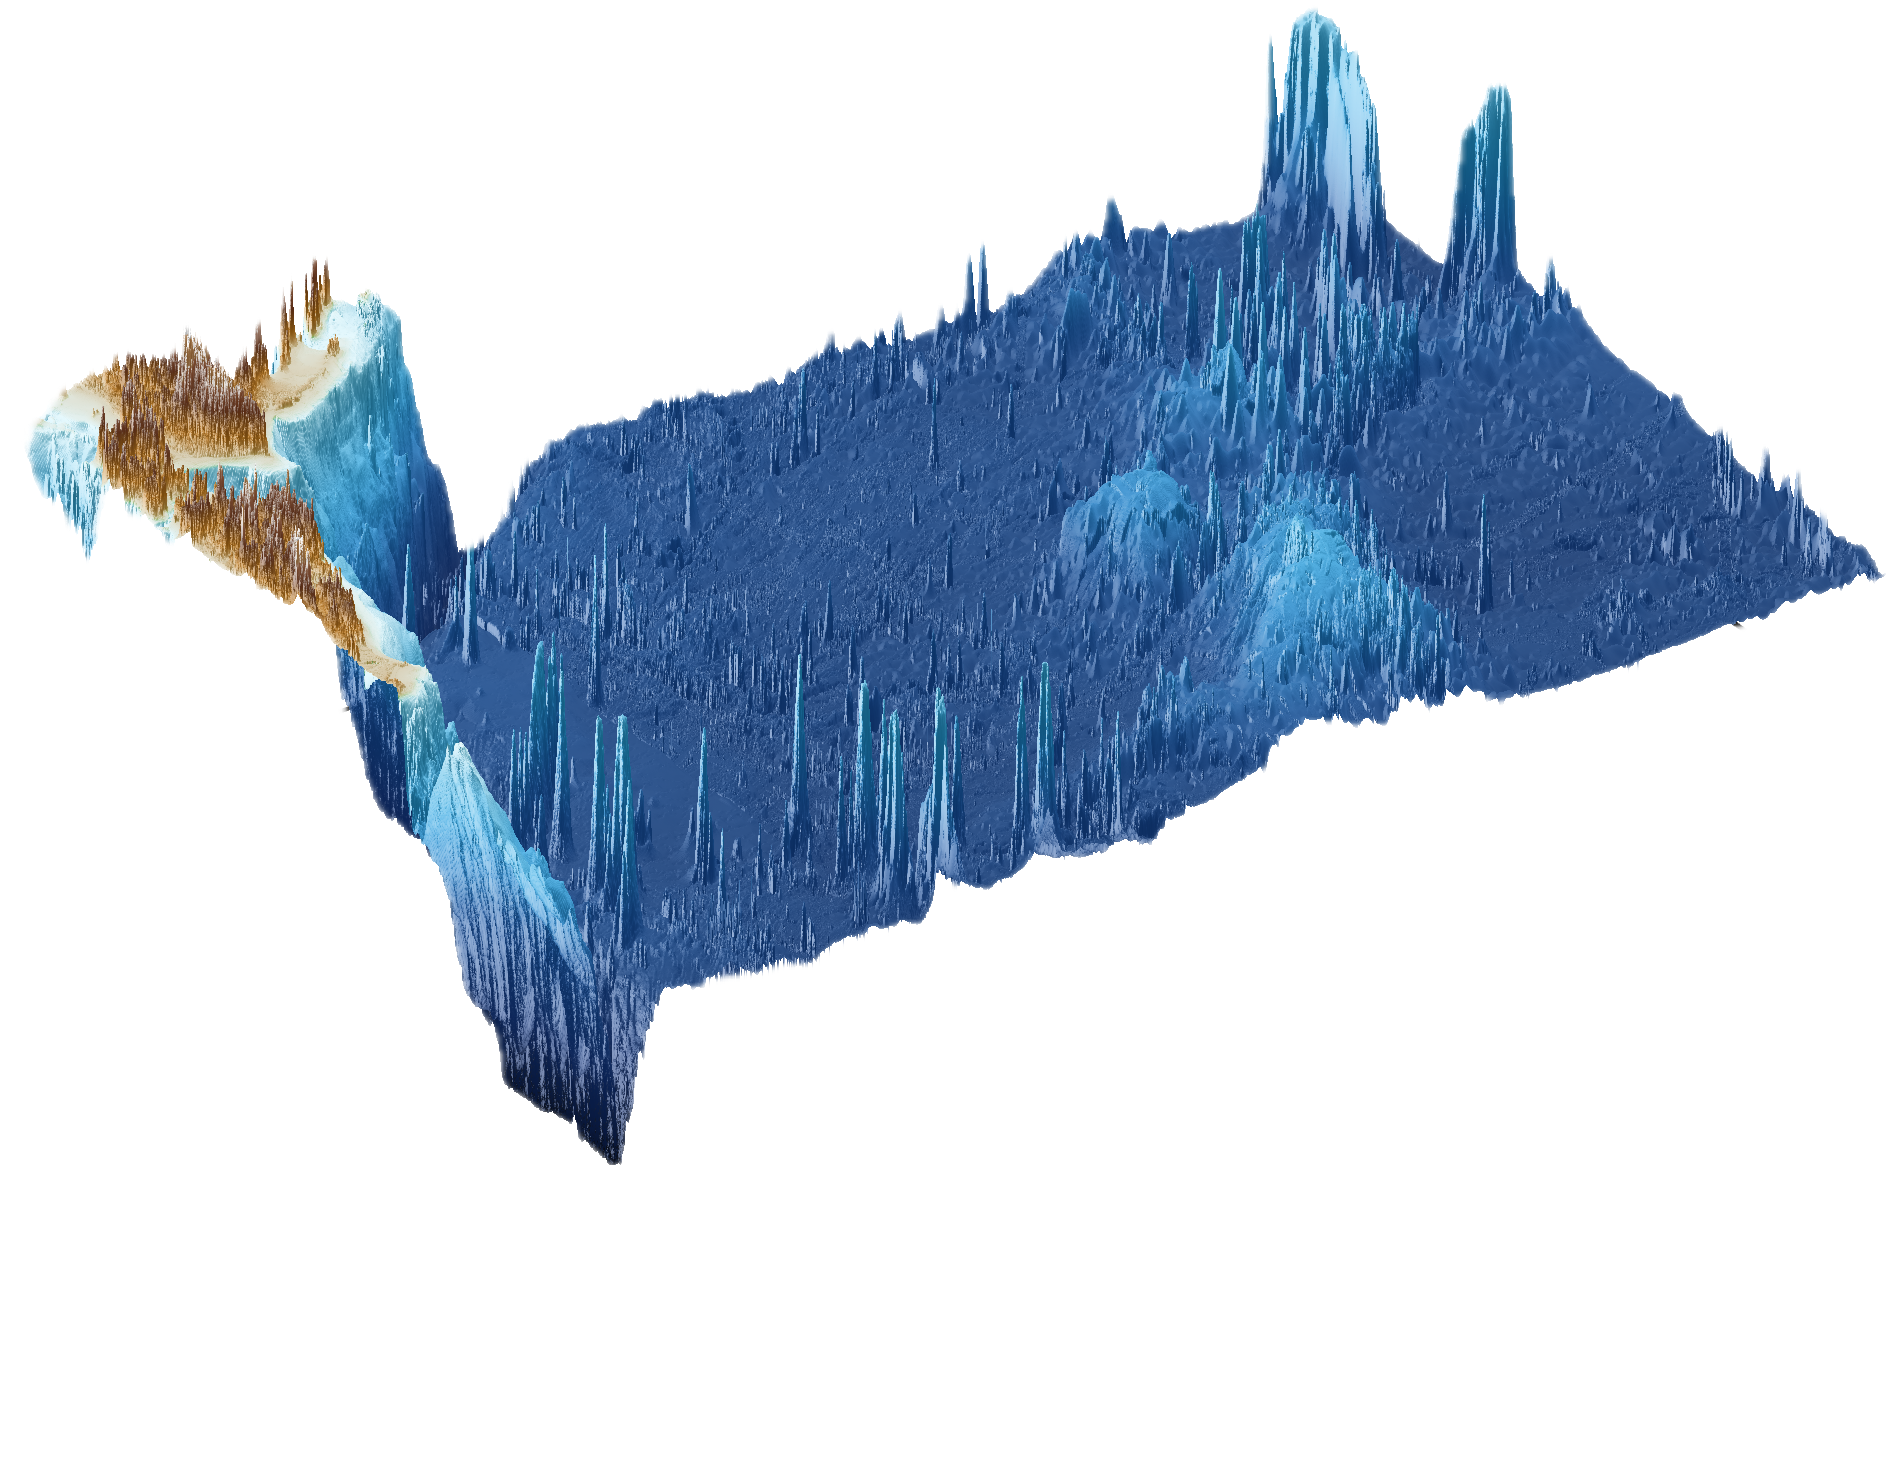
\includegraphics[width=0.5\linewidth]{tohoku_karte.png} \\
  {\large \textbf{Tohoku 2011} \;\textbullet\; \textbf{Chile 1960}}\\[0.25cm]
  {\small\color{foam!85} Ladbar als Szenario, auf Basis \textcolor{teal}{echter Erdbebenparameter}.}
  \note{~40s. Macht aus der Spielwiese etwas Validierbares. Wichtig fuers gemischte Publikum.}
\end{frame}

% ---------- 6 | Architektur + Abschluss ------------------------------
\begin{frame}{Wie es läuft}
  \vspace{0.7cm}
  \centering
  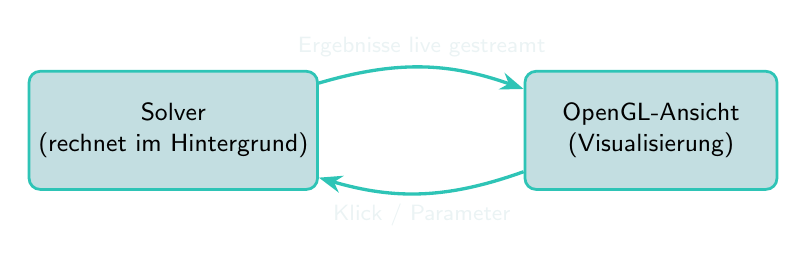
\begin{tikzpicture}[
      block/.style={draw=teal, line width=1pt, rounded corners,
        fill=ocean!25, text=black, align=center, font=\small,
        minimum width=3.2cm, minimum height=1.5cm},
      pfeil/.style={-{Stealth}, teal, line width=1.2pt}]
    \node[block] (solver) {Solver\\(rechnet im Hintergrund)};
    \node[block, right=2.6cm of solver] (render) {OpenGL-Ansicht\\(Visualisierung)};
    \draw[pfeil] (solver) to[bend left=18]
      node[above, midway, foam!85, font=\footnotesize] {Ergebnisse live gestreamt} (render);
    \draw[pfeil] (render) to[bend left=18]
      node[below, midway, foam!85, font=\footnotesize] {Klick / Parameter} (solver);
  \end{tikzpicture}
  \\[1.1cm]
  {\LARGE\bfseries Kein Video. Keine Aufzeichnung.\\[0.2cm]
   Ein Klick. Der \textcolor{teal}{Ozean reagiert}.}
  \note{~40s. Technik bewusst knapp. Rueckbezug auf die Eingangsfrage. Details fuer Fragerunde.}
\end{frame}

\end{document}